\documentclass[11pt]{report}
% PACKAGES
  \usepackage[a4paper,left=28mm,right=28mm,top=30mm,bottom=30mm]{geometry}
  \usepackage{graphicx,epstopdf}      % Used to import external graphics (figures)
  \usepackage{hyperref}       % Used for referring to links inside and outside the document
  \usepackage[table]{xcolor}  % To include colors 
  \usepackage{amsmath}        % For most of the math symbols and environments (such as \begin{align})
  \usepackage{amssymb}        % For using symbols in the document
  \usepackage{float}          % Arranging of figures on the page
  \usepackage[bf]{caption}    % Arranging the captions in floating environments [bf] makes the Figures bold
  \usepackage{subcaption}     % To arrange captions of subfigures
  \usepackage{booktabs}       % For standard tabular tables, with rules
  \usepackage{tabularx}       % For clean tables such as in the Nomenclature
  \usepackage{fancyhdr}       % Fancy headers
  % \usepackage[colorinlistoftodos]{todonotes}      % To create todo notes
  \usepackage[nottoc,notlot,notlof]{tocbibind}    % Add bibliography to content
  \usepackage{bm}             % Make bold symbols
  \usepackage{lipsum}
  \usepackage{parskip}
  \usepackage[export]{adjustbox}
  \usepackage{changepage}
% LAY-OUT
  % \usepackage{pdfpages}

  % \usepackage{pdflscape}

   \renewcommand\thesection{\arabic{section}}

  % \usepackage[mathletters]{ucs}
  % \usepackage[utf8x]{inputenc}
  %Bibliography for references, with reference style options
  \usepackage[
  backend=biber,
  bibstyle=ieee,
  citestyle=numeric-comp,
  dashed=false,
  url = false,
  maxnames=8,
  maxcitenames=2,
  mincitenames=1,
  sorting=none,
  isbn = false,
  doi = false
  ]{biblatex}
  \addbibresource{references.bib}

  %Set the page style
  \pagestyle{fancy}
  \fancyhead[L]{\ifodd\value{page} \slshape\nouppercase{\rightmark} \else \fi}
  \fancyhead[R]{\ifodd\value{page} \else \slshape\nouppercase{\leftmark} \fi}
  \chead{ }
  \lfoot{}
  \rfoot{}
  \cfoot{\small\thepage}


  %Give colors to links/refs etc
  \hypersetup{colorlinks, linkcolor={blue!0!black}, 
                          citecolor={blue!70!black}, 
                           urlcolor={blue!80!}} 
                       
  %% Set up numbering and spacing
  \numberwithin{equation}{section}        %Number the equations per section
  \numberwithin{figure}{section}          %Number the figures per section
  \numberwithin{table}{section}           %Number the tables per section
  \captionsetup[table]{skip=1pt}          %Skip 1 pt after a table
  \captionsetup[figure]{skip=3.5pt}       %Skip 4 pt after a figure
  \setcounter{secnumdepth}{3}             %Count up to the subsubsection 
  \setcounter{topnumber}{1}               %Number of floats at top of a page (default is 2)

  %%%%% proof/theorem/definition boxes

  \usepackage{cleveref}
  \usepackage[most]{tcolorbox}
  \newtcbtheorem{Theorem}{Theorem}{
    enhanced,
    sharp corners,
    attach boxed title to top left={
      yshifttext=-1mm
    },
    colback=white,
    colframe=blue!75!black,
    fonttitle=\bfseries,
    boxed title style={
      sharp corners,
      size=small,
      colback=blue!75!black,
      colframe=blue!75!black,
    } 
  }{thm}

  \newtcbtheorem{Definition}{Definition}{
    enhanced,
    sharp corners,
    attach boxed title to top left={
      yshifttext=-1mm
    },
    colback=white,
    colframe=blue!25,
    fonttitle=\bfseries,
    coltitle=black,
    boxed title style={
      sharp corners,
      size=small,
      colback=blue!25,
      colframe=blue!25,
    } 
  }{def}

  \newtcbtheorem[no counter]{Proof}{Proof}{
    enhanced,
    sharp corners,
    attach boxed title to top left={
      yshifttext=-1mm
    },
    colback=white,
    colframe=blue!25,
    fonttitle=\bfseries,
    coltitle=black,
    boxed title style={
      sharp corners,
      size=small,
      colback=blue!25,
      colframe=blue!25,
    } 
  }{prf}
% DEFINITIONS
  %% Titlepage definitions
  \newcommand{\deltitle}{Impact-Aware Control for a Dual-Arm Setup}      %Your project title
  \newcommand{\StudentName}{Gijs van den Brandt}  %Student name
  \newcommand{\StudentID}{1257110}                    %Your student number
  % \newcommand{\DCcode}{2021.109}                      %Get your DC code from the D&C secretariat

  %% Operators
  \DeclareMathOperator\sign{sgn}                      %Sign function
  \DeclareMathOperator\diag{diag}                     %Diagonal operator
  \DeclareMathOperator\imag{Imag}                     %Imaginary part of complex variable
  \DeclareMathOperator\real{Real}                     %Real part of complex variable
  \DeclareMathOperator*{\argmin}{\arg\!\min}          %Argmin operator
  \newcommand{\norm}[1]{\left\lVert#1\right\rVert}    %Norm operator

  %% Variable definition
  \newcommand{\R}{\mathbb{R}}                         % Set of real numbers
  \newcommand{\C}{\mathbb{C}}                         % Set of complex numbers

\begin{document}

% Summary 
  \section*{Progress meeting 9 | 7 October, 2022}


  \section*{1. Progress}
  \begin{itemize}
  \item \textbf{Impact detection:} As discussed last time, I was taking a closer look at Benn's impact detector as this supposedly was what Sven also ended up using. While doing so, I could not find any reason for why Benn looks at force estimations for impact detection rather than velocity measurements. Sven provides the reason that, during some timesteps, velocity measurements are missing. This is not the case for the force estimations due to the first order filter. I don't find this a valid argument as a similar filter could also be applied to the velocity measurements. Furthermore there are other benefits to impact detection using velocity, which I explain in section \ref{sec:impact}. I will get in touch with Benn to see if he (or perhaps you) can convince me that force-based impact detection is more suitable for reference spreading than velocity-based impact detection.
    
  \item \textbf{Learning from demonstration:} In section \ref{sec:lfd}, I propose two controllers that track ante- and post impact references learned from the demonstration: an impedance controller, and a force/position controller as was used by Sven. 
  The impedance controller is better at replicating the demonstration in a scenario with high repeatability (i.e., impact occurs at the same time as during demonstration) and can be used for a large variety of tasks (grabbing/twisting/etc). The force position controller is better at adjusting to objects of different sizes, though it does lose some versatility in which tasks it can perform. I figure that, for the goal of depelatization that I have in mind, the geometry and inertia of the boxes does not differ between demonstration and replication (thought their position may differ slightly). Furthermore I would like to not only perform grabbing tasks where the force mostly acts in orthogonal direction, but also a sliding task with shear forces. Therefore, the impedance controller is more appropriate than the position/force controller.

  \item \textbf{Velocity reference:} Until now, the teleoperation controller received position and orientation data from the VR device. Performing fast object manipulation tasks could benefit from also using a velocity reference, as this makes the controller more responsive. Therefore I added this feature to the dual arm controller. This change is barely noticeable for rotations, but transnational tracking is now much better, and I was also able to decrease the impedance stiffness which I previously put very high to overcome friction. Some more tuning is still required, as currently the robot's safety limits are sometimes exceeded when the VR device is moved to quickly. This seems to be 

  \item \textbf{Custom end effector:} After some silicone delivery delays, the second custom end effector is now completed. As previously requested by Alessandro, I will try to record some videos where I pick up heavy objects with two soft end effectors before the upcoming meeting.

  \end{itemize}
\newpage
  \section*{2. Agenda}
  During the meeting, I would like to discuss the following points:

  \begin{itemize}
      \item Do you agree with my arguments for using velocity-based impact detection instead of force-based impact detection? 
      \item Given the usecase of boxes with constant geometry/inertia between demonstration and replication, the impedance controller is more suitable than the force/position controller. Should I also consider other options?
      \item The safety limit issues occur mostly with rotation, which had me wondering what kind of stiffness Sven was using for rotation. I was unable to find anything regarding control of the rotational DoF's in Sven report. Do you more about his approach in this regard? Did he perhaps prescribe a reference in rotation?
  \end{itemize}

  \section*{3. Next steps}

  \begin{itemize}
      \item Ensure that controller with velocity reference does not exceed safety limits
      \item Apply LfD controller on dual-arm setup
      \item Write background section for the final report
  \end{itemize}

  \section*{4. Long-term planning}
  Below is the current long-term planning for the project phase. The description of the labeled subjects are given in the preparation phase report and are also provided on the next page.

  \begin{figure}[H]
  \centering
  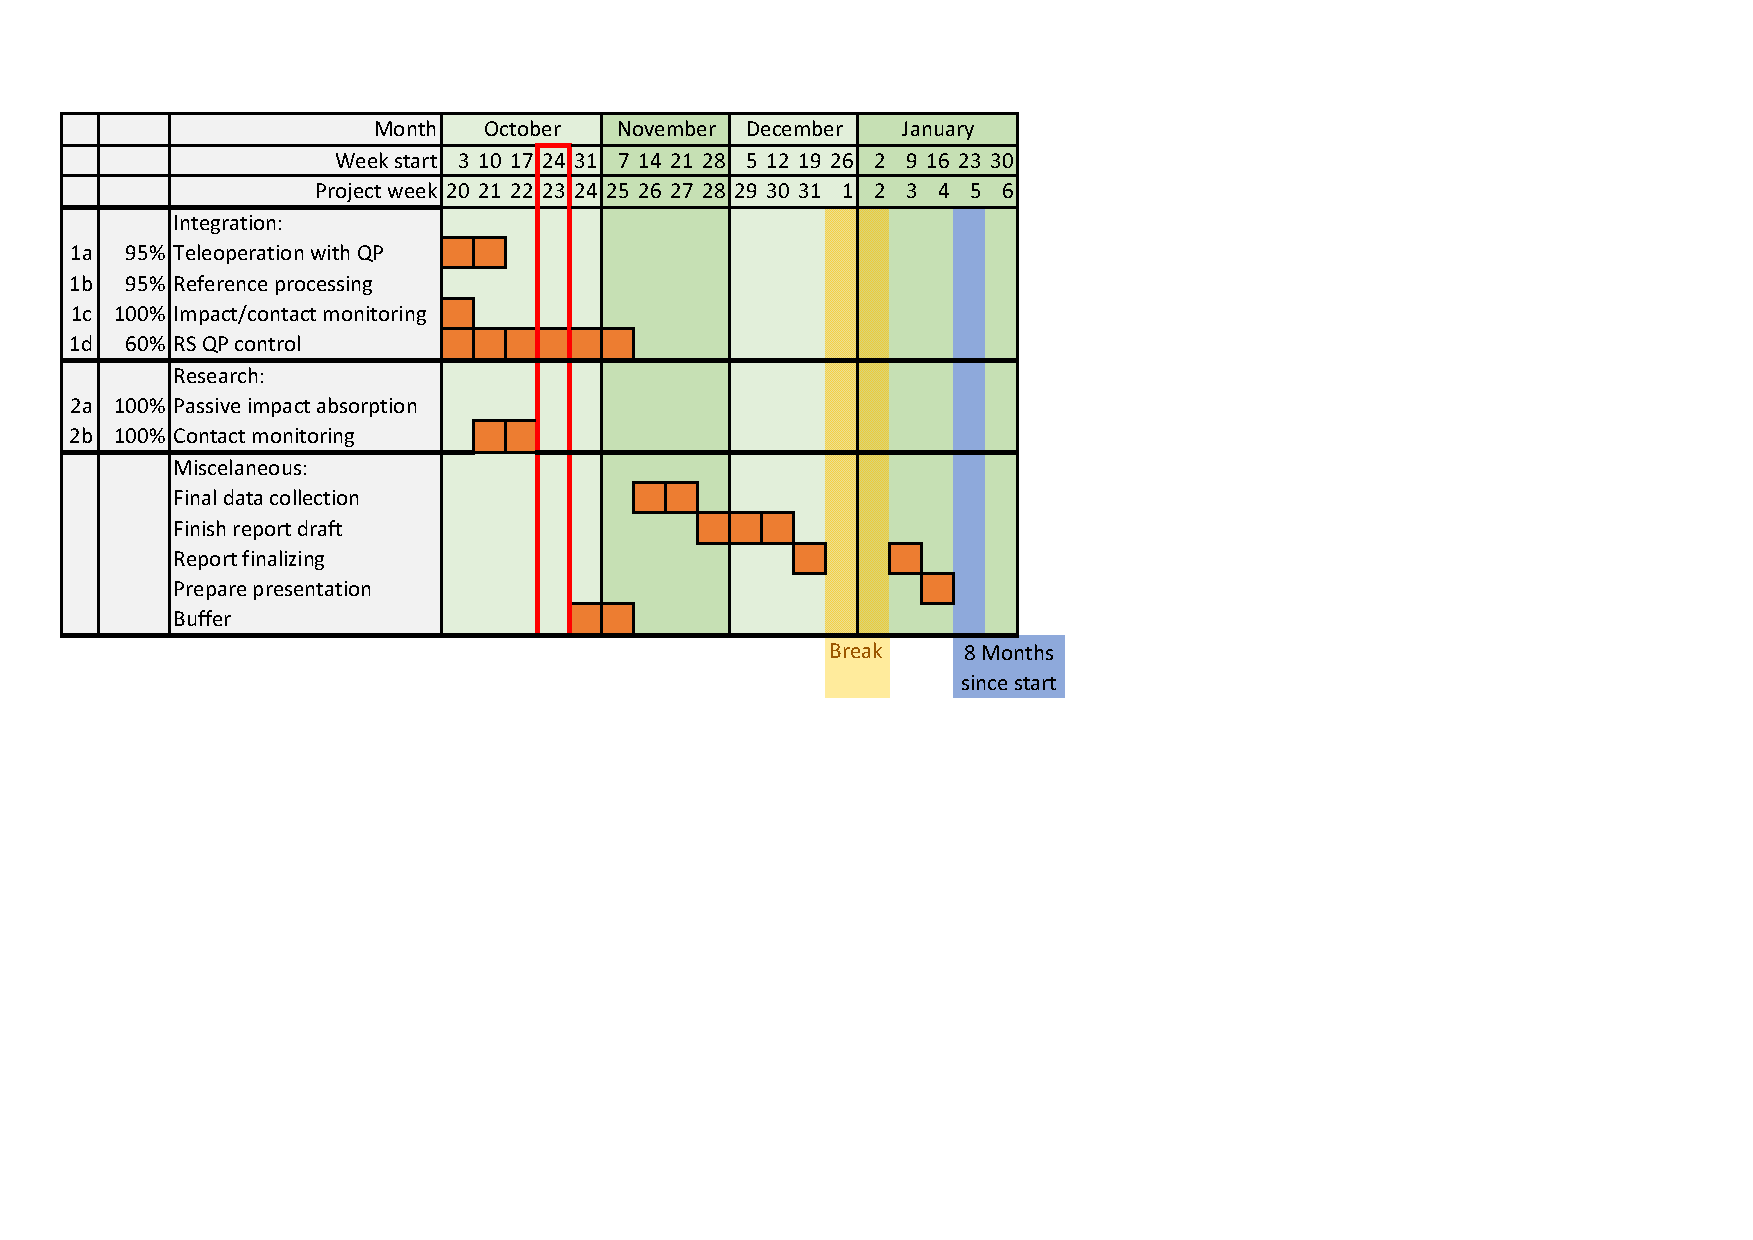
\includegraphics[width=0.7\textwidth, trim={0.87cm 9.5cm 10cm 1.5cm},clip]{Graphics/planning v2.pdf}

  \label{fig:my_label}
  \end{figure}

  \begin{enumerate}
  \item[1a] \textbf{Translating dual-arm teleoperation to the physical setup.} The existing implementation in simulation already uses the mc\_rtc interface, meaning that the switch to reality shouldn't pose an issue. Nevertheless, this step also involves getting familiar with the software, which increases the anticipated time for this step.
  \item[1b] \textbf{Extracting references from the demonstration data.} The demonstrated trajectories should be split into ante-impact and post-impact sections, and extended to facilitate RS. Furthermore multiple measurements should be used to fit ProMPs, after which a reference can be generated. It is also key to identify which data should be learned from the demonstration. This is not limited to choosing between a force or position reference, but can also consists of learning properties of the environment, e.g. friction cones or box inertia, that are crucial to a dual-arm box grabbing scenario.
  \item[1c] \textbf{Integrating impact detection and contact monitoring in mc\_rtc.} The majority of the impact detector's complexity resides in the momentum observer; however, Franka Emika's software already has an integrated momentum observer. This still leaves tuning of the impact detecting algorithms which might be time consuming. Furthermore an analysis comparing the available methods could be worthwhile. Factors which determines the effectivity of the impact detection algorithm include speed of detection, as well as reliability, i.e. the rate of false positives. The addition of objects that cause unexpected impacts is not considered a part of the research scope.
  \item[1d] \textbf{Configuring QP controllers for the ante-impact, intermediate, and post-impact phase.} For each of the phases, it is important to address the redundancy in the arms' degrees of freedom. After that, control for the ante-impact phase should be trivial. For the intermediate phase, it is expected that ante-impact reference tracking without velocity feedback should be applicable on a dual-arm robot, though this might prove to be false, in which case other methods should be investigated. During post-impact control, the challenge will be maintaining non-slip contact with the box. It is difficult to say how well the results from simulations can be repeated with torque control, where the state of the box can not be sensed to be used in the QP controller.
   \item[2a] \textbf{Passive impact absorption:} A soft cover for the end effector will be designed. Such a cover can be connected to the Panda by connecting bolts to the so-called flange interface. A mold will be created using 3D printing to allow for casting of various silicone soft covers. Design parameters -- i.e. material properties (controlled by choosing different kinds of silicone) and soft cover thickness -- will be analyzed experimentally. A systematic comparison between various designs will require an experiment plan including a realistic testing scenario. Evaluation of performance can be based on the oscillatory response in position and force after establishing contact. Furthermore multiple scenarios with various box surface properties and robot poses should be considered.
  
  \item[2b] \textbf{Contact monitoring:} When investigating contact monitoring, two approaches can be taken: either using proprioceptive or exteroceptive sensors. A possible improvement for contact monitoring using proprioceptive sensors could be to wait a fixed time starting from the last detected impact, rather than waiting a fixed time from the first impact. As for exteroceptive sensors, they can be a hurdle for large-scale commercial applications as they are not integrated in the robot. However, if a soft cover is to be mounted to the end effector, including tactile sensors for impact and contact monitoring becomes more feasible. Practical questions such as which tactile sensor to use and how to integrate it could be addressed, though this is not absolutely necessary for completing the research goals, and therefore has a low priority.
  \end{enumerate}
% main text
  \newpage
  \section{Impact detection using contact force vs velocity}\label{sec:impact}
  For impact detection, Benn and Sven considered two options: looking at jumps in velocity, or jumps in force. Ultimately, Benn and Sven both ended up using the forces, whereas I think looking at velocities makes more sense in the context of reference spreading. This section explains my reasoning.

  Looking at jumps in force for impact detection could result in false positives. Consider an end effector that is already exerting a contact force on a fixed surface using impedance control. A jump in the reference would result in a jump in the contact force. Even if contact is maintained throughout the event, the jump in contact force would trigger the impact monitor while no impact has actually occurred. In the described situation, the velocity remains unchanged, meaning that a velocity-based impact detector would not return a false positive.

  Additionally, contact forces cannot be directly measured, and the process of estimating them with a momentum observer is quite complex and involves a delay when compared to determining the velocity. 

  Given the downsides of looking at force rather than velocity, there must be significant benefits to warrant using force estimates for impact detection. I am not able to fully identify Benn's reasoning here (he states that "The most common method of impact detection is through the use of external joint torque estimators", though I suspect this is in the context of human safety). Sven, however, does provide an argument. In his experiments, he noticed that velocity data was missing during some timesteps, which resulted in poor impact detection. The impact detector using force did not suffer from this issue.

  As discussed during the questions of Sven's defense, the momentum observer acted as a filter which made it so that missing data was not problematic for the impact detector that uses force. Therefore I don't think that missing velocity data is a valid argument for looking at force data; applying a filter to account for missing velocity data makes more sense in my opinion.

  As a final argument, the reason for applying reference spreading is diminishing peaks in the velocity tracking error. If a jump in velocity cannot be measured, then it is also not possible for the velocity tracking error to peak (barring a peak in the reference). While there is some connection between the peaking error and contact forces, the connection between measured velocity and the peaking error is much closer.

  Conclusively, based on the arguments given above, a velocity-based impact detector is more appropriate for reference spreading than a force-based impact detector.
  
  \newpage

  \section{Learning impedance vs force/position reference}\label{sec:lfd}
  When considering what reference to extract from demonstrations, two options come to mind. Firstly, it is possible to look at the position trajectory of the robot during demonstration. As the robot position by itself does not fully describe the robot's state, a force reference should also be extracted. This resembles the approach used by Sven. A second option would be to learn an impedance reference, i.e., the position of the VR device, which encapsulates both position and force. This section describes how both approaches would be implemented for a simple testcase. Based on this, a decision is made on whether impedance or force/position control is more suitable for impact-aware learning from teleoperation.

  As a disclaimer, it should be noted that neither Sven's implementation nor the current VR implementation utilize a velocity reference. While Sven used reference spreading for the force reference, the value of reference spreading might be more apparent when applied to a velocity reference. The tracking performance is also expected to improve with the addition of a velocity reference. Therefore, the remainder of this section will assume that a velocity reference is included in the control scheme. Obtaining this reference should not prove difficult as a robot's velocity can easily be determined, and the HTC Vive provides velocity (and even acceleration) measurements.

  \subsection{Testcase description}
  The testcase consists of a 1-dof system with mass $m=1$ kg and position $x$. The EoM is given by $m\ddot{x}=F_c+F_e$, with control force $F_c$ and environmental contact force $F_e$ following

  $$F_e=\begin{cases}
    0 & \text{if } x\geq w\\
    -k_e x-d_e \dot{x}               & \text{if } x<w.
  \end{cases}$$
  Parameters $k_e=10^4$ N/m and $d_e=100$ Ns/m represent the environment's contact stiffness and damping, respectively. Furthermore, $w$ describes the location of the contact surface and is equal to $0$ m unless stated otherwise.

  The control force during the demonstration, $F_c^d$, is generated using an impedance controller with stiffness $k_c=40$ N/m and damping $d_c=2\sqrt{k_c}$ Ns/m:

  $$ F_c^d = k_c(y-x)+d_c(\dot{y}-\dot{x}).$$

  The references $u$ and $\dot{y}$ emulate an input coming from the VR device.

  Figure \ref{fig:1d_demonstration} shows the reference $y$, together with simulation results of the demonstration. Five signals from this simulation are saved, so that they may be used as a reference for the LfD controllers: $y$, $\dot{y}$, $x^d$, $\dot{x}^d$, and $F_e^d$. Superscript $d$ denotes a result from the demonstration simulation.

  \begin{figure}[]
  \centering
  \begin{adjustwidth}{0pt}{5pt}
  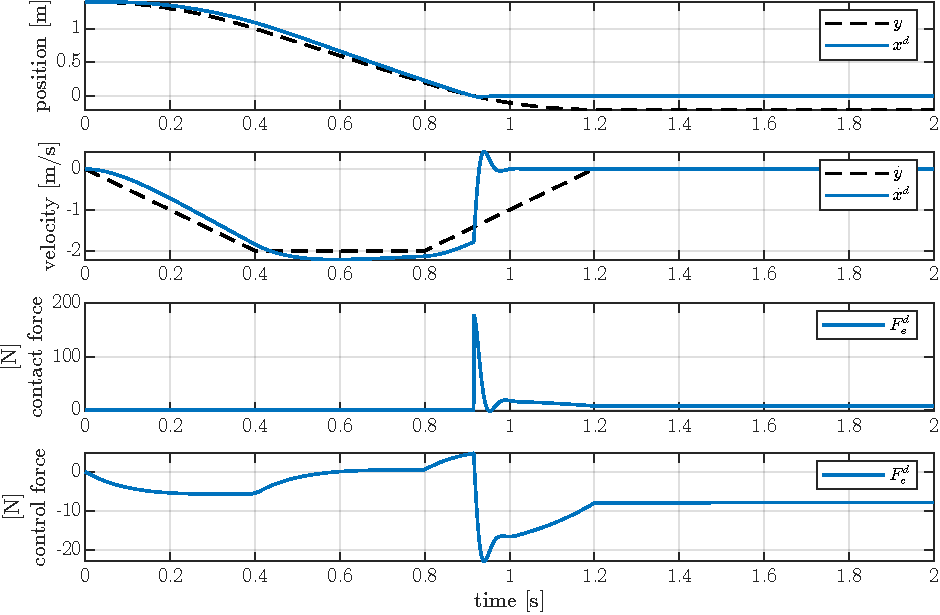
\includegraphics[right]{Graphics/1d_demonstration.pdf}
  \end{adjustwidth}
  \caption{Results of the demonstration simulation}
  \label{fig:1d_demonstration}
  \end{figure}

  \begin{figure}[]
  \centering
  \begin{adjustwidth}{0pt}{5pt}
  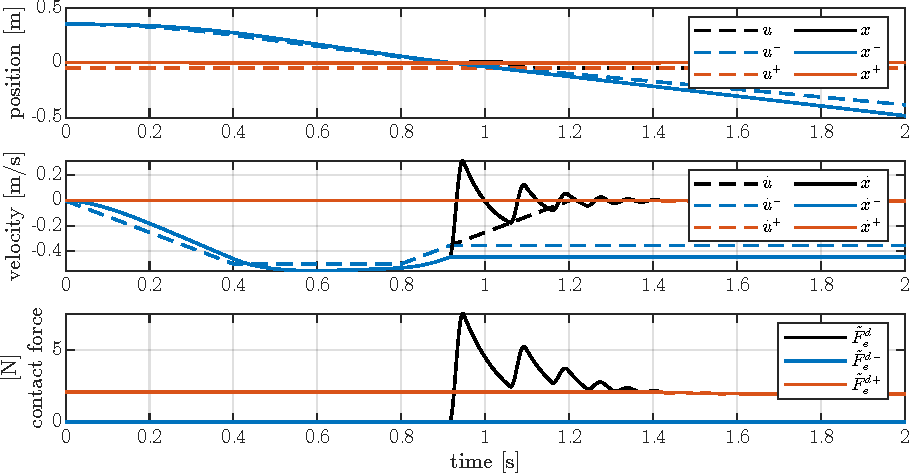
\includegraphics[right]{Graphics/1d_RS.pdf}
  \end{adjustwidth}
  \caption{Ante- and post-impact references generated from the demonstration data}
  \label{fig:1d_RS}
  \end{figure}

  \subsection{Reference spreading}
  To apply reference spreading, the references must be split into an ante- and post-impact reference, and extended. The resulting references are shown in Figure \ref{fig:1d_RS}. The ante-impact reference is extended after the time of impact, defined as the first timestep where $x\leq d$. Furthermore, the post-impact references are extended up to 0.5 seconds after time of impact. This delay prevents extension during an oscillation. Force and velocities were extended with a constant hold, whereas positions were updated to match the new velocity references.


  \subsection{LfD controllers}
  Two controllers will be compared. The impedance controller $F_c^i$ is identical to the controller used in demonstration, i.e.,
  $$ F_c^i = k_c(y-x)+d_c(\dot{y}-\dot{x}).$$
  Furthermore, the force/position control force $F_c^f$ is given by
  $$ F_c^f = k_c(x^d-x)+d_c(\dot{x}^d-\dot{x}) + F_e^d.$$  
  This force/position controller is identical to what Sven used, with the exception that Sven did not use a velocity reference $\dot{x}^d$. (He does fit a reference to the velocity, but it is not used by his controller according to his paper/thesis. Could this perhaps be an oversight?)% In the absence of a velocity reference, reference spreading does not contribute to performance. This contradicts the conclusions of Sven's thesis, though I believe the difference Sven noticed was a matter of inaccurate impact detection.)

  These controllers were evaluated with the switching references from the previous subsection. Firstly, it will be assumed that the location of the contact surface matches the location during the demonstration, i.e., $w=0$ m. The results are shown in Figure \ref{fig:1d_learned_w0}.

  When comparing the impedance controller during demonstration and during reference spreading, tracking of position and velocity is very similar. There is a notable difference in control force however. Since the velocity reference is set to zero by reference spreading, the resulting peak in control force is smaller. 

  The difference between the force/position controller and impedance controller is very minor. The force/position controller does not directly follow $u$, but follows $x^d$ instead, causing it to slightly lag behind the impedance controller, giving it a slight disadvantage.

  In another experiment, the contact surface is moved to $w=0.1$ m when executing the learned reference. This is shown in Figure \ref{fig:1d_learned_w01}. This experiment gives similar results, in the sense reference spreading results in reduced control force peaks compared to during the demonstration, and the impedance controller outperforms the position/force controller in tracking the position during the demonstration.

  \subsection{Conclusion/discussion}
  Given the experimental results, the impedance controller barely outperforms the force/position controller. Combined with the fact that the force/position controller is adds complexity -- in the sense that a force reference is required and that the controller deviates from the controller used during the demonstration -- the impedance controller is deemed more suitable for the impact-aware learning from teleoperation usecase.

  Jari lead me to understand that a force/position controller could have benefits with a slightly different implementation. Currently, if the impact surface is closer than expected, this results in a larger contact force. If the position tracking was disabled after impact, the force reference would ensure that the contact force is not affected by the position of the contact surface. In a multidimensional case, position tracking shouldn't necessarily be disabled in all directions. This direction may differ between different tasks however, therefore taking away from the controllers versatility.

  % other conclusions:
  % - for the impedance controller, reference spreading makes basically no difference if a velocity reference is not used.
  % - for position/force controller without velocity reference, reference spreading makes little difference compared to a simple 1st order lowpass filter applied to the force reference.

  \begin{figure}[!h]
  \centering
  \begin{adjustwidth}{0pt}{5pt}
  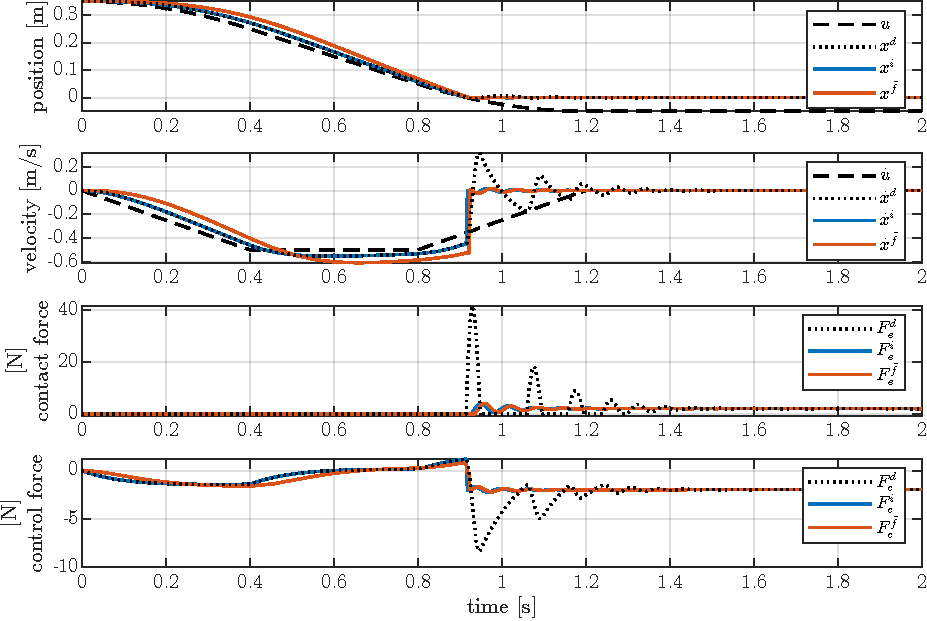
\includegraphics[right]{Graphics/1d_learned_w=0.pdf}
  \end{adjustwidth}
  \caption{Results of both LfD controllers using RS. Impact at $x=0$ m}
  \label{fig:1d_learned_w0}
  \end{figure}

  \begin{figure}[!h]
  \centering
  \begin{adjustwidth}{0pt}{5pt}
  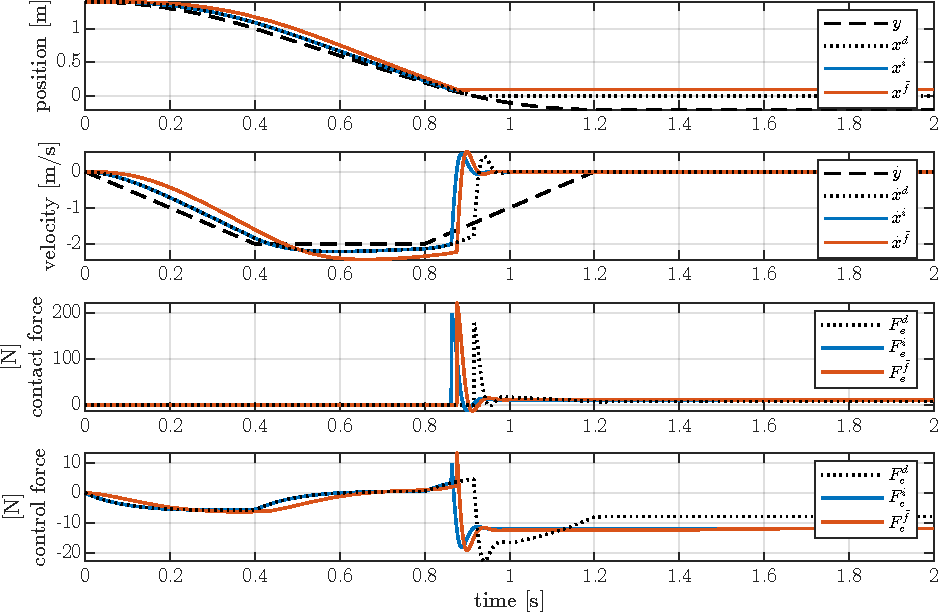
\includegraphics[right]{Graphics/1d_learned_w=0.1.pdf}
  \end{adjustwidth}
  \caption{Results of both LfD controllers using RS. Impact at $x=0.1$ m}
  \label{fig:1d_learned_w01}
  \end{figure}
\newpage
  \subsection{Extra: value of reference spreading in absence of velocity reference}
  The experiment was repeated using controllers that do not use a velocity reference. This was done with reference spreading (Figure \ref{fig:1d_learned_w01_novel}) and without reference spreading (Figure \ref{fig:1d_learned_w01_novel_nors}). For the impedance controller, there is no noticeable difference between using reference spreading or not using it. For the force/position controller, reference spreading ensure that the force reference does not activate prior to impact, which can be interpreted as a small improvement. Nevertheless, the effects of reference spreading isn't nearly as significant as it is in the presence of a velocity reference.


  \newpage
  \begin{figure}[!h]
  \centering
  \begin{adjustwidth}{0pt}{5pt}
  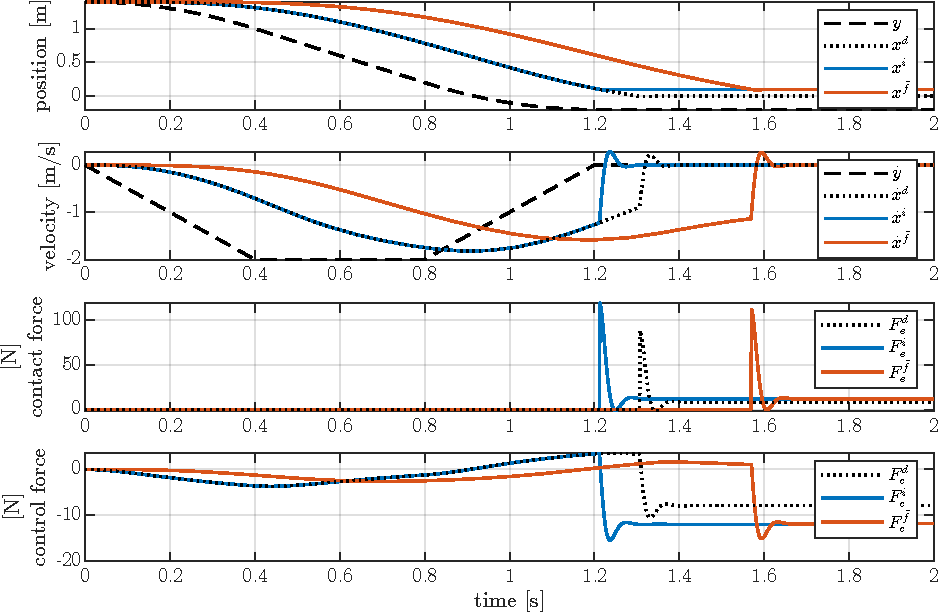
\includegraphics[right]{Graphics/1d_learned_w=0.1_novel.pdf}
  \end{adjustwidth}
  \caption{Results using RS without a velocity reference. Impact at $x=0.1$ m}
  \label{fig:1d_learned_w01_novel}
  \end{figure}

  \begin{figure}[!h]
  \centering
  \begin{adjustwidth}{0pt}{5pt}
  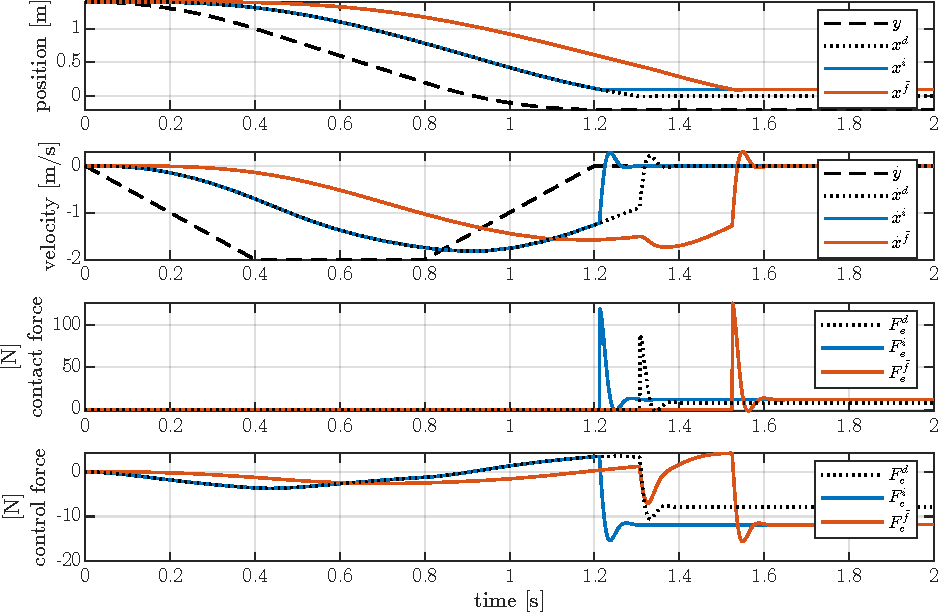
\includegraphics[right]{Graphics/1d_learned_w=0.1_novel_nors.pdf}
  \end{adjustwidth}
  \caption{Results without RS and without a velocity reference. Impact at $x=0.1$ m}
  \label{fig:1d_learned_w01_novel_nors}
  \end{figure}
  % These controllers were evaluated in an ideal scenario, meaning that the impact occurs at the exact same time as it did during the demonstration, and there is a perfect estimation of $F_e^d$. The results are shown in Figure \ref{}. 

  % For the impedance controller, the results exactly match the demonstration as there is no difference between the controllers. 

  % The position/force controller shows drastically different behavior however. Already in the ante-impact phase where the force reference is still zero, the controller tracks $x^d$ which tracked $u$, meaning that $x^p$ will always lag behind. This could be improved by directly tracking $u$ in the ante-impact phase.

  % Furthermore, at the moment of impact, the force controller tries to track the peak in the force trajectory while, at the same time, the impact itself also causes a peak in force. As a result, $F_e^p$ spikes to approximately $2F_e^i$ at impact. After impact, contact loss due to bouncing is far more evident in $x^p$ than it is in $x^i$. Despite these results, the force/position controller should not yet be disregarded without looking at a situation where reference spreading is required.

  % In a less ideal scenario, estimation $\tilde{F}_e^d$ is a first-order filtered version of $F_e^d$ following

  % $$\dot{\tilde{F}}_e^d = k_f(F_e^d-\tilde{F}_e^d)$$

  % with gain $k_f=10$ s$^{-1}$, and  $\tilde{F}_e^d(0) = F_e^d(0)$. The filtered signal is shown in Figure \ref{fig:my_label}. This change does not affect the impedance controller, however the force/position controller shows significantly improved results in Figure \ref{fig:my_label}, since the filter removes peaks in the force reference. 

% BIBLIOGRAPHY

  \newpage
  \addcontentsline{toc}{chapter}{References}
  \printbibliography[title=References]

  % \newpage
  % \thispagestyle{empty} \ \newpage


\end{document}